\section{Simulations - détails}

\begin{frame}{Simulations - Architecture}
    \begin{figure}
      \centering
      \resizebox{0.5 \columnwidth}{!}{
        \begin{tikzpicture}
          \path
            +(90:10) node (a) {\includegraphics[page=5, trim=0cm 24cm 32cm 0cm, clip]{img/mute-figures.pdf}}
            +(-90:10) node (b) {\includegraphics[page=5, trim=0cm 24cm 32cm 0cm, clip]{img/mute-figures.pdf}}
            +(180:5) node (c) {\includegraphics[page=5, trim=0cm 24cm 32cm 0cm, clip]{img/mute-figures.pdf}}
            ++(0:10)
            +(90:10) node (d) {\includegraphics[page=5, trim=0cm 24cm 32cm 0cm, clip]{img/mute-figures.pdf}}
            +(-90:10) node (e) {\includegraphics[page=5, trim=0cm 24cm 32cm 0cm, clip]{img/mute-figures.pdf}}
            +(0:5) node (f) {\includegraphics[page=5, trim=0cm 24cm 32cm 0cm, clip]{img/mute-figures.pdf}};

          \draw[latex-latex, line width=1.5mm]
            (a) edge (b) (a) edge (c) (a) edge (d) (a) edge (e) (a) edge (f)
            (b) edge (c) (b) edge (d) (b) edge (e) (b) edge (f)
            (c) edge (d) (c) edge (e) (c) edge (f)
            (d) edge (e) (d) edge (f)
            (e) edge (f);
        \end{tikzpicture}
      }
    \end{figure}
    \begin{itemize}
      \item \alert{10 noeuds} éditent collaborativement un document
      \item Topologie \alert{réseau entièrement maillée}
      \item Ne considère \alert{pas de pannes ou de pertes de message}
    \end{itemize}
  \end{frame}

  \begin{frame}{Simulations - Modifications}
    \metroset{block=transparent}
    \begin{block}{Se décompose en 2 phases}
      \begin{enumerate}
        \item \alert{Génération du contenu} (80\% d'\ins, 20\% de \rmv)
        \item \alert{Édition} (50/50\%)
      \end{enumerate}
      Noeuds passent à la phase 2 quand leur copie locale atteint une taille donnée (15 pages - 60k caractères)
    \end{block}
    \textbf{Nombre d'opérations : } 15k par noeud, 150k au total
  \end{frame}

  \begin{frame}{Simulations - Mécanisme de renommage}
    \metroset{block=transparent}
    Noeuds \alert{utilisent LogootSplit} (LS) ou \alert{RenamableLogootSplit} (RLS)
    \begin{block}{Noeuds de renommage}
      \begin{itemize}
        \item 1 à 4 noeuds effectuent une \alert{opération \ren toutes les 30k opérations}
        \item Opérations \ren générées à un point donné sont \alert{concurrentes}
      \end{itemize}
    \end{block}
  \end{frame}

